% THIS IS SIGPROC-SP.TEX - VERSION 3.1
% WORKS WITH V3.2SP OF ACM_PROC_ARTICLE-SP.CLS
% APRIL 2009
%
% It is an example file showing how to use the 'acm_proc_article-sp.cls' V3.2SP
% LaTeX2e document class file for Conference Proceedings submissions.
% ----------------------------------------------------------------------------------------------------------------
% This .tex file (and associated .cls V3.2SP) *DOES NOT* produce:
%       1) The Permission Statement
%       2) The Conference (location) Info information
%       3) The Copyright Line with ACM data
%       4) Page numbering
\pagenumbering{arabic}
% ---------------------------------------------------------------------------------------------------------------
% It is an example which *does* use the .bib file (from which the .bbl file
% is produced).
% REMEMBER HOWEVER: After having produced the .bbl file,
% and prior to final submission,
% you need to 'insert'  your .bbl file into your source .tex file so as to provide
% ONE 'self-contained' source file.
%
% Questions regarding SIGS should be sent to
% Adrienne Griscti ---> griscti@acm.org
%
% Questions/suggestions regarding the guidelines, .tex and .cls files, etc. to
% Gerald Murray ---> murray@hq.acm.org
%
% For tracking purposes - this is V3.1SP - APRIL 2009

\documentclass{acm_proc_article-sp}

\usepackage{url}
\usepackage{booktabs}

\begin{document}

\title{The Article/Editor Ranking : Bringing Order to Wikipedia}
%\subtitle{[Extended Abstract]
%\titlenote{A full version of this paper is available as
%\textit{Author's Guide to Preparing ACM SIG Proceedings Using
%\LaTeX$2_\epsilon$\ and BibTeX} at
%\texttt{www.acm.org/eaddress.htm}}}
%
% You need the command \numberofauthors to handle the 'placement
% and alignment' of the authors beneath the title.
%
% For aesthetic reasons, we recommend 'three authors at a time'
% i.e. three 'name/affiliation blocks' be placed beneath the title.
%
% NOTE: You are NOT restricted in how many 'rows' of
% "name/affiliations" may appear. We just ask that you restrict
% the number of 'columns' to three.
%
% Because of the available 'opening page real-estate'
% we ask you to refrain from putting more than six authors
% (two rows with three columns) beneath the article title.
% More than six makes the first-page appear very cluttered indeed.
%
% Use the \alignauthor commands to handle the names
% and affiliations for an 'aesthetic maximum' of six authors.
% Add names, affiliations, addresses for
% the seventh etc. author(s) as the argument for the
% \additionalauthors command.
% These 'additional authors' will be output/set for you
% without further effort on your part as the last section in
% the body of your article BEFORE References or any Appendices.

\numberofauthors{3} %  in this sample file, there are a *total*
% of EIGHT authors. SIX appear on the 'first-page' (for formatting
% reasons) and the remaining two appear in the \additionalauthors section.
%
\author{
% You can go ahead and credit any number of authors here,
% e.g. one 'row of three' or two rows (consisting of one row of three
% and a second row of one, two or three).
%
% The command \alignauthor (no curly braces needed) should
% precede each author name, affiliation/snail-mail address and
% e-mail address. Additionally, tag each line of
% affiliation/address with \affaddr, and tag the
% e-mail address with \email.
%
% 1st. author
\alignauthor
Maximilian Klein\\
       \affaddr{OCLC Research}\\
       \affaddr{777 Mariners Island Blvd}\\
       \affaddr{San Mateo, CA, 94404}\\
       \email{kleinm@oclc.org}
% 2st. author
\alignauthor
Thomas Maillart\\
       \affaddr{School of Information}\\
       \affaddr{ University of California, Berkeley, 102 South Hall}\\
       \affaddr{Berkeley, CA 94720}\\
       \email{thomas.maillart@ischool.berkeley.edu}
% 3rd. author
\alignauthor
John Chuang\\
       \affaddr{School of Information}\\
       \affaddr{ University of California, Berkeley, 102 South Hall}\\
       \affaddr{Berkeley, CA 94720}\\
       \email{chuang@ischool.berkeley.edu}
}


\date{23 February 2014}
% Just remember to make sure that the TOTAL number of authors
% is the number that will appear on the first page PLUS the
% number that will appear in the \additionalauthors section.

\maketitle
\begin{abstract}
We introduce a new method to jointly rank the quality of articles and the expertise
 of editors in Categories of Wikipedia, based on the bi-partite network information 
 of who has contributed at least once to an article on the one hand, and what are 
 the articles that have edited at least once by a given author on the other hand.
  We show that this ``reflexive" ranking method exhibits high correlations with 
  usual article quality and user expertise metrics, which account for quality on 
  Wikipedia (that we assume to be a grand truth here). In particular, we find that 
  the quality of an article can be captured very well by our method right after a few 
  edits, while the expertise of editors is captured increasingly better over time. 
  Our results suggest that it is easier to predict the quality of an article from the 
  editors who touched it, rather than editor expertise from articles they have 
  edited.
\end{abstract}

% A category with the (minimum) three required fields
\category{H.4}{Information Systems Applications}{Miscellaneous}
%A category including the fourth, optional field follows...
\category{D.2.8}{Software Engineering}{Metrics}[complexity measures, performance measures]

\terms{to be completed}

\keywords{to be completed, if necessary} % NOT required for Proceedings

\section{Introduction}
From product reviews to online collaboration platforms, the World Wide Web is increasingly populated with knowledge contributed by the crowds. One positive aspect is the immediate sharing of information, which in turn helps others take more informed decisions about the quality of a product, the cleanliness of a restaurant, whether it is worth buying a book. But the reliability of the contribution is limited by the level of expertise of the person who made the contribution. In many case, repeated contributions of the same type by several individuals (e.g., reviews) average out idiosyncracies (assuming that individual do not influence each others). Many crowd sourcing mechanisms have been designed in this way \cite{}. The reliability/quality of a contribution is however more critical  when the same contribution is not necessarily repeated, or repeatable. Open source collaboration projects face such an issue: rewriting several times Wikipedia or the whole open source software codebase would be simply be impossible. Yet these open collaboration projects can achieve remarkable quality \cite{nature paper}. This is achieved through {\it peer-production} a labor organization, which mainly relies on two main ingredients : (i) task self-selection and (ii) peer-review : individuals choose the tasks they believe they are more qualified for, and they review the work of others also according to their skills \cite{benkler2002}. These rules have been initially used for open source software development \cite{raymond1999}, for which it is possible to ultimately test the quality of the work by executing the code. However, for natural language knowledge, like  Wikipedia, there is no ``machine" to execute the code. Therefore the quality of knowledge remains subjective, and it is mainly tied to the expertise of the person in the domain of contribution, and to the number of persons (and their respective expertise) who have contributed to a piece of knowledge (e.g., an article). The level of expertise in one domain can in turn be approximated by the number of related articles contributed by the same individual, and so on. 

On Wikipedia, is there a way to assess relative quality of both articles and editors by only considering whose editor has touched which article ? This is the problem we are addressing in this paper. 

The rest of this paper is organized as follows. With begin with discussion of related work, followed by a description of the method. We then present the results and conclude. 

\begin{figure}[!t]
\centering
%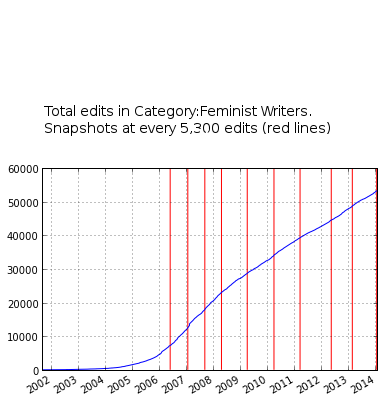
\includegraphics[width=0.9\columnwidth]{accumulative snapshot points for Feminist Writers.png}.
\caption{Matrix}
\label{fig:triangle_matrix}
\end{figure}


%Theory of ranking  \cite{Blumm2012}

%\subsection{criticism of alternative economy}
%we are not really saying much about how the economy of wikipedia, i.e. inputs and outputs.
%
%but still we can say something about the fact peer production, is indeed different from tradition economy.
%
%but still might be useful to justify why we are using HH model, and what we expect as differences. 

%\subsection{criticism of improving rankings approach}
%no reliable metrics for ranking people, there is never a benchmark to say that we have a "BETTER" metric in terms of measuring quality, precisely because we use those to calibrate.

%but still can say it is an effecient alternative metric, 

%\subsection{issue of possible overfitting}
%how do we justify the existence of alpha and beta as the parameters we calibrate

\section{Related Work}
The model we present here is deeply influenced by a recent stream of research in economics that aims at explaining the GDP of countries based on the nature of goods they produce and export. The first model was proposed by \cite{hidalgo2007,hidalgo2009}, and reworked by 
	
A network analysis of countries� export flows: firm grounds for the building blocks of the economy \cite{caldarelli2012network}; A new metrics for countries' fitness and products' complexity \cite{tacchella2012new}; Measuring the Intangibles: A Metrics for the Economic Complexity of Countries and Products \cite{cristelli2013measuring}; Economic complexity: Conceptual grounding of a new metrics for global competitiveness \cite{tacchella2013economic}; Competitors� communities and taxonomy of products according to export fluxes
  \cite{cristelli2012competitors}
  
The model proposed by Caldarelli et al. \cite{caldarelli2012network} is a sort of two-dimensional PageRank algorithm \cite{pagerank}. Instead of jumping from web page to webpage, the random walker goes from country to products, and from products to countries.

We then applied the most general implementation of the $\mathbf{FQ}$ algorithm as developed for modelling the economy and competitiveness of countries. The $\mathbf{FQ}$ is a nonlinear generalization of the Hidalgo Hausman "Reflections Method". \cite{Caldarelli}. The algorithm has both a stochastic, iterative implementation, and an analytic solution. We demonstrate the iterative solution, to gain some intuition for the algorithm.

\begin{equation}
\begin{cases}
 w^*_c = A(\sum^{N_p}_{p=1} M_{cp}k_p^{-\alpha})k_c^{-\beta} \\
w^*_p = B(\sum^{N_c}_{c=1} M_{cp}k_c^{-\beta})k_p^{-\alpha}
\end{cases}
\end{equation}

At each iterative step we simultaneously rank editor "fitness", and article "ubiquity". In the linear model, the first iteration of "fitness" is the sum of articles to which that editor has contributed, and the "ubiquity" is the sum of editor who have contributed to that article. In the second iteration, say a user is as fit as the average the ubiquities of the of the pages edited. But this is all things being equal.

In the economic domain, the best products are those that are made by the fewest countries. Therefore in our average we want to give more weight to those best producing countries. This measure of good contributors being more important to success, is measured by alpha. A higher alpha means that a good product needs to be exported by the best countries. In Caldarelli, to correlate best with GDP rankings alpha = 1.5 Our result we find the  opposite - negative values of alpha. in the not competitive but collaborative wikipedia, where the best articles are produced by the highest number of editors

\section{Method}
While it relies on the same principles as in \cite{caldarelli2012network}, our proposed model is conceptually different : our ``products" are Wikipedia articles, which are not the basis for competitions but rather for cooperation. Editors enrich the articles together to make best articles. However, like countries, editors have limited capabilities and limited resources (e.g., time), which force them make choices on their contributions.

The matrix $\mathbf{M}$ shown in Figure \ref{fig:triangle_matrix} shows when an article has changed at some point by a given editor. The matrix is ordered on both dimensions by decreasing order of editors who have changed more articles (vertical axis) and by decreasing order of articles that have been changed by most editors (horizontal axis) for a category of Wikipedia articles (here Feminist Writers). Although it is a rough count, the matrix tells already about the experience of an editor in the given category, and the attention an article has gotten from editors, which is an implicit quality measure according to the second principle of peer-production : peer-review. This count is the zero order of the Article/Editor ranking algorithm, and thus the initiation step is given by 

\begin{equation}
\begin{cases}
 w^{0}_{editors}(\alpha , \beta) = \sum_{articles} \mathbf{M}_{editors,articles} \\
 w^{0}_{articles}(\alpha , \beta) = \sum_{editors} \mathbf{M}_{editors,articles} 
\end{cases}
\end{equation}

Now, let's consider the second step :  if an article has been changed by editors who edited more articles, then the quality of the article should be higher. Similarly, if an editor has edited articles that have been edited by more editors, then the expertise of the editor should be higher (the only reason for making this claim is the collaborative nature of Wikipedia, and learning by imitation). Accordingly, the third step is the following : if an article has been changed by editors who edited more articles that have edited by more editors, then the quality of the article should be higher. Similarly, if an editor has edited articles that have been edited by more editors that have edited more articles, then the expertise of the editor should be higher. The algorithm goes on recursively, incorporating the quality (resp. expertise) information of the article (resp. editor) at the previous step. 

{\bf tell about the stochastic process here} \cite{caldarelli2012network}

{\bf say that it is a ranking algorithm. We care only about the ranking of articles and editors}

The algorithm at step $n$ then writes,

\begin{equation}
\begin{cases}
 w^{n+1}_{e}(\alpha , \beta) = \sum\limits_{a}\mathbf{G}_{e,a}(\beta)w^{n}_{a}(\alpha , \beta) \\
 w^{n+1}_{a}(\alpha , \beta) = \sum\limits_{e}\mathbf{G}_{a,e}(\beta)w^{n}_{e}(\alpha , \beta) 
\end{cases}
\end{equation}
\begin{equation}
\begin{cases}
\mathbf{G}_{e,a}( \beta)  = \frac{\mathbf{M}_{e,a}k_{e}^{-\beta}}   {\sum_{e'=1}\mathbf{M}_{e',a}k_{e'}^{-\beta}} \\
\mathbf{G}_{a,e}(\alpha)  = \frac{\mathbf{M}_{e,a}k_{a}^{-\alpha}}   {\sum_{a'=1}\mathbf{M}_{e,a'}k_{a'}^{-\alpha}}\end{cases}
\end{equation}

As shown on Figure \ref{fig:convergence}, the algorithm converges in a non-trivial way, because they can be reduced ergodic Markov chains. In the iterative solution we see how certain editors start low, but then climb in rankings. This means that they are editing few articles, but those articles are less ubiquitous. We see a lot of top ranked editors drop very quickly at first, because its we don't 

and an analytical solution can be found :

\begin{equation}
\begin{cases}
w^*_e = A(\sum\limits_{a=1} \mathbf{M}_{e,a}k_a^{-\alpha})k_e^{-\beta} \\
w^*_a = B(\sum\limits_{e=1} \mathbf{M}_{e,a}k_e^{-\beta})k_a^{-\alpha}
\end{cases}
\end{equation}

that we use onwards.


\begin{figure}[!t]
\centering
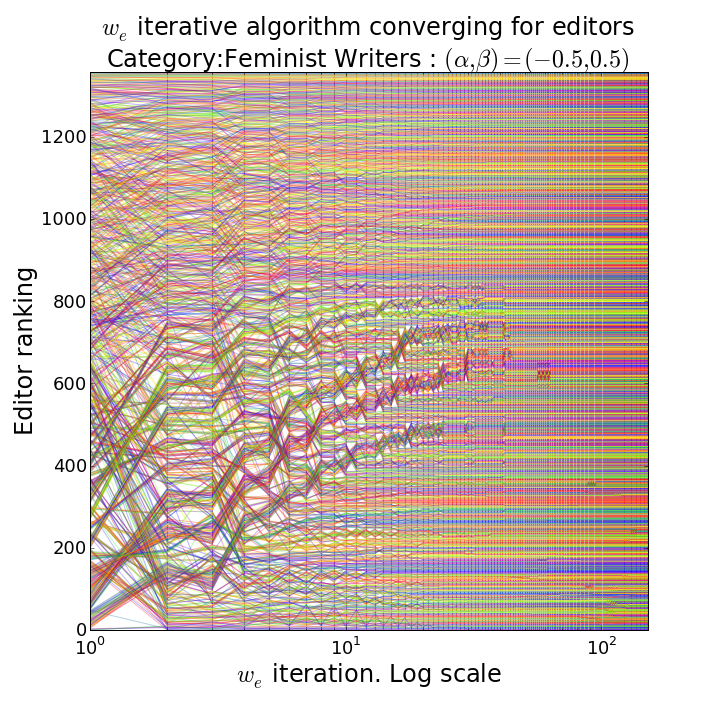
\includegraphics[width=0.9\columnwidth]{Figures/fem_editors_iter_converge.png}.
\caption{Convergence of $w_e$}
\label{fig:convergence}
\end{figure}

%With some imagination Wikipedia, and many other online collaborative projects can be viewed as such a market. (Here we only consider English Wikipedia). We consider Wikipedia Editors to be our "countries", and Wikipedia Articles to be "products". Therefore a country producing a product is interpreted as an editor editing an article. We also inherit the assumption that the better editors will be those who edit the rarer articles, although we re-adjust that assumption in instructive ways later on. 


%2. We develop a new measure for the degree of collaborativity of category.

%Questions. Can this economics theory be applied, into other "economies"? Which is the other side of a Wikipedia question, which is "What are better ways to rank Wikipedia editor and articles, since the flawed Edit Counts and Article Metrics, are used as proxies"?


\section{Data}
The main input of the Article/Editors ranking algorithm is the matrix $M$ which determines, for a category on Wikipedia, which articles have modified at least once by each editor. We collected contribution data for articles in 10 categories (c.f. table \ref{tab:statistics} for summary statistics on the categories). In addition, we made 10 snapshots of equal number of edits to account for the evolution over time of each category (see Figure \ref{fig:accumulative_snapshots}
).

\begin{tabular}{llll}
\toprule
Category & Users & Articles &  Edits \\
\midrule
2013 films &  5215 &     1896 &  150956 \\
American male novelists &  9946 &     2460 &  224783 \\
American women novelists &  5968 &     1936 &  138716 \\
Bicycle parts &   210 &       70 &    4981 \\
Computability theory &   272 &       92 &    7117 \\
Counterculture festivals &   578 &       66 &   10515 \\
Economic theories &  1145 &      212 &   28658 \\
Feminist writers &  1357 &      233 &   25738 \\
Military history of the US &   854 &      180 &   20172 \\
Nobel Peace Prize laureates &  4165 &      104 &   91522 \\
Sexual acts &  2190 &       93 &   45901 \\
Yoga &   730 &      123 &   25315 \\
\bottomrule
\label{tab:statistics}
\end{tabular}

\begin{figure}[!t]
\centering
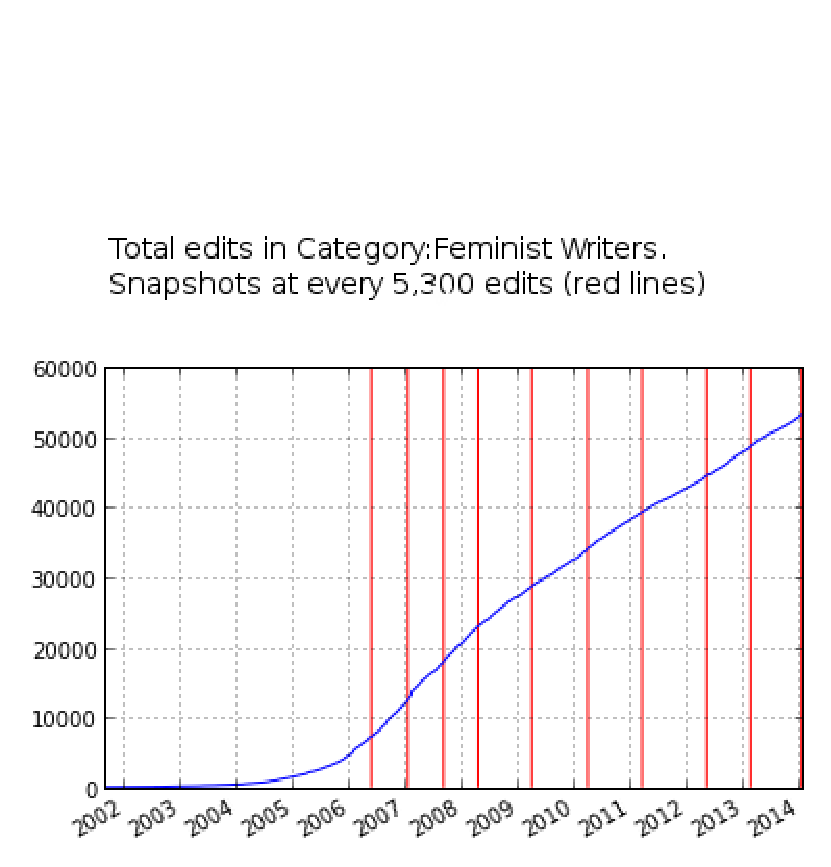
\includegraphics[width=0.9\columnwidth]{Figures/cumulative_snapshots_Feminist_Writers.eps}
\caption{cumulative snapshots Feminist Writers eps }
\label{fig:figure1}
\end{figure}

 For each snapshot, we constructed the matrix $\mathbf{M_{e,a}}$ of contributors versus edited articles, similar to the country versus products matrix of the Economics Domain. For each snapshot, the values in $\mathbf{M_{e,a}}$ are defined as the number of edits made by editor $e$ on article $a$ in the category occurring in the snapshot time. Note that the final snapshot represents the entire history of the category up to the present date.
  
The matrix $\mathbf{\hat{M}_{e,a}}$ is a binary representation of $\mathbf{M_{e,a}}$ where each nonzero entry is replaced with $1$. This represents if editors have touched which articles rather than how much they have touched each article. In the economics domain, the distinction of making a binary matrix out of the data is interpreted an alternative metric to GDP per capita, rather than GDP. Here we could also see the distinction as normalized editor fitness. It has a typical triangular structure as shown on Figure \ref{fig:triangular_matrix}. The matrix $\mathbf{\hat{M}_{e,a}}$ constitutes the basic input for implementing the Biased Markov Chain Approach, which we will call the $\mathbf{w^*}$ algorithm, which is an analytic solution to the iterative $\mathbf{W}$ algorithm. \cite{Caldarelli} 

The exogenous metric for editors $v_e$ we take is $labour hours$. For each editor the contribution history upto the snapshot point,  divide into strings of $edit sessions$, edits that occur within 1 hour of the previous edit. Then $labour hours$ are determined by subtracting the looking at the total time between the first and last edit in each edit session, and then summing the labours of each edit session. \cite{Geiger, Halfaker}. 

For an exogenous measure of article quality, $ v_a$,  we use a group of 5 text analysis metrics performed on Wikipedia articles at the lastest time in the snapshot. These are ratio of mark-up to readable text, number of headings, article length, citations per article length, and outgoing intrawiki links. To reduce the dimensionality of these 5 metrics, we perform Principal Component Analysis, and accept the principal component. Variance explained by the first principal component, was as high as .7 and never below .5 http://www-users.cs.umn.edu/~morten/publications/wikisym2013-tellmemore.pdf, http://mailer.fsu.edu/~bstvilia/papers/quantWiki.pdf \cite{ Morten}.




%For each snapshot, we constructed the matrix $\mathbf{M_{e,a}}$ of contributors versus edited articles, similar to the country versus products matrix of the Economics Domain. For each snapshot, the values in $\mathbf{M_{e,a}}$ are defined as the number of edits made by editor $e$ on article $a$ in the category occurring in the snapshot time. Note that the final snapshot represents the entire history of the category up to the present date. 

\subsection{Interpretation of w* algorithm in the context of open collaboration}

To understand the results, we must have a firm grasp on what $\alpha$ and $\beta$ mean. They are more easily understood by roughly rewriting $\mathbf{w^*}$ as:
\begin{equation}
\begin{cases}
w^{*}_{e} \sim k^{1-\beta}_{e} \langle k_{a}^{-\alpha}\rangle_e \\

w^{*}_{a} \sim k^{1-\alpha}_{a} \langle k_{e}^{-\beta}\rangle_a
\end{cases} \label{eqsim}
\end{equation}

where $\langle k_{a}^{-\alpha}\rangle_e$ is the arithmetic average of k  $k_{a}^{-\alpha}$. 

Since we see beta and alpha are close to being additive inverses, we can just study what it means for them to increase and decrease.

For Editors.
As beta approaches one from infinity then editors are less judge by their the amount of contributions and more about the quality of the articles they contribute to. As beta becomes more negative below one, then the amount of articles is more important in predicting success.  So 'gnomier' editors are more successful in this case. So we can see beta as a style marker for a category.

The lower beta, the more a diversified editor will be successful in a Category, and the higher beta, the more a targeted quality-writing author will be successful.


\subsection{Theory of Ranking in Open Collaboration}
How this would used in an setting

\subsection{How do w* algorithm should behave in open collaboration (theory)}

It might be opposite or negative.

\subsection{Data}
1. The current investigation involved collecting historical data of edition and quality metrics, from 10 categories of articles in English Wikipedia, with focus on fine-grained edits by contributors to articles.

2. The chosen categories contain between 50 and 4000 articles, and between 50 and 5000 contributors have edited at least 100,000 times all the articles over their history. (c.f. table \ref{tab:statistics} for summary statistics on the categories). 

3. For each category, we constructed 10 accumulative snapshots, that is each starting from the first edit in the category until 10\% more of the categories total edits have occurred. \ref{fig:accumulative_snapshots}

\begin{tabular}{llll}
\toprule
Category & Users & Articles &  Edits \\
\midrule
2013\_films &  5215 &     1896 &  150956 \\
American\_male\_novelists &  9946 &     2460 &  224783 \\
American\_women\_novelists &  5968 &     1936 &  138716 \\
Bicycle\_parts &   210 &       70 &    4981 \\
Computability\_theory &   272 &       92 &    7117 \\
Counterculture\_festivals &   578 &       66 &   10515 \\
Economic\_theories &  1145 &      212 &   28658 \\
Feminist\_writers &  1357 &      233 &   25738 \\
Military\_history\_of\_the\_United\_States &   854 &      180 &   20172 \\
Nobel\_Peace\_Prize\_laureates &  4165 &      104 &   91522 \\
Sexual\_acts &  2190 &       93 &   45901 \\
Yoga &   730 &      123 &   25315 \\
\bottomrule
\label{tab:statistics}
\end{tabular}

\begin{figure}[!t]
\centering
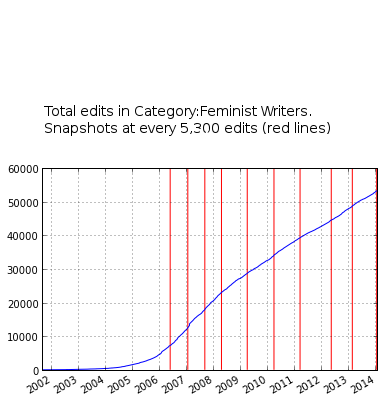
\includegraphics[width=0.9\columnwidth]{accumulative snapshot points for Feminist Writers.png}.
\caption{Cumulative snapshots, Feminist Writer}
\label{fig:cumsnaps}
\end{figure}

 For each snapshot, we constructed the matrix $\mathbf{M_{e,a}}$ of contributors versus edited articles, similar to the country versus products matrix of the Economics Domain. For each snapshot, the values in $\mathbf{M_{e,a}}$ are defined as the number of edits made by editor $e$ on article $a$ in the category occurring in the snapshot time. Note that the final snapshot represents the entire history of the category up to the present date.


The matrix $\mathbf{\hat{M}_{e,a}}$ is a binary representation of $\mathbf{M_{e,a}}$ where each nonzero entry is replaced with $1$. This represents if editors have touched which articles rather than how much they have touched each article. In the economics domain, the distinction of making a binary matrix out of the data is interpreted an alternative metric to GDP per capita, rather than GDP. Here we could also see the distinction as normalized editor fitness.


The output of $\mathbf{w^*}$ are a pair of rankings $ w^*_e$ and $ w^*_a$ for editors and articles respectively.

\begin{equation}
\begin{cases}
w^*_e = A(\sum^{N_a}_{a=1} M_{e,a}k_a^{-\alpha})k_e^{-\beta} \\
w^*_a = B(\sum^{N_e}_{e=1} M_{e,a}k_e^{-\beta})k_a^{-\alpha}
\end{cases}
\end{equation}

Next we collect exogenous metrics as comparison for both  $w^{*}_{e}$ and $w^{*}_{a}$, which we call  $v_e$ and $v_a$.

It is important to note that we are not competing with these metrics, but take them as state-of-the-art, Grand Truth, to which we calibrate against. We adopt a "less is more" approach. We using the exogenous variable to proxy 

Yes, indeed for authors, what we are measuring is a weaker proxy for the gnomieness.

but for artilces the exogenous metric is quite, good, i.e. similar to what we are measuring


\subsection{Testing against Wikipedia Metrics}
We turn to the evaluation of the method against metrics 

\begin{itemize}
  \item 
  \item 
\end{itemize}


Having our endogenous and exegenous variables now, we perform a recursive grid search over the two dimensions of $\alpha$ and $\beta$ to find a maximum correlation between our rankings from $\mathbf{w^*}$ and our exogenous variables. Our grid search operates on the interval $[-5,5]$ with a resolution of 0.2 in on each axis. Importantly we search for negative values of $\alpha$ and $\beta$, which is not done in the Economics Domain. t

\subsection{Finding trends}

5. While the implementation presented here is strictly similar to \ref{}, the interpretation is slightly different in the context of group collaboration. Indeed, while countries competes for selling products, the hypothesis here is that Wikipedia contributors cooperate, at least in a very informal way, for improving the quality of articles.

\section{Results}




\section{Discussion}

6. {\it Refer to problems here, if any.}


The exogenous metric for editors $v_e$ we take is $labour hours$. For each editor the contribution history upto the snapshot point,  divide into strings of $edit sessions$, edits that occur within 1 hour of the previous edit. Then $labour hours$ are determined by subtracting the looking at the total time between the first and last edit in each edit session, and then summing the labours of each edit session. \cite{Geiger, Halfaker}. 

For an exogenous measure of article quality, $ v_a$,  we use a group of 5 text analysis metrics performed on Wikipedia articles at the lastest time in the snapshot. These are ratio of mark-up to readable text, number of headings, article length, citations per article length, and outgoing intrawiki links. To reduce the dimensionality of these 5 metrics, we perform Principal Component Analysis, and accept the principal component. Variance explained by the first principal component, was as high as .7 and never below .5 http://www-users.cs.umn.edu/~morten/publications/wikisym2013-tellmemore.pdf, http://mailer.fsu.edu/~bstvilia/papers/quantWiki.pdf \cite{ Morten}.


\subsection{Calibrating}

Having our endogenous and exogenous variables now, we perform a recursive grid search over the two dimensions of $\alpha$ and $\beta$ to find a maximum correlation between our rankings from $\mathbf{w^*}$ and our exogenous variables. Our grid search operates on the interval $[-5,5]$ with a resolution of 0.2 in on each axis.


We also use a maximizing algorithm to find the values of $\alpha$ and $\beta$ which maximize the spearman $\rho$ rank correlation between our endogenous and exogenous rankings. This is performed for both of internal users ranks versus labour hours and internal article ranks and aggregated actionable article metrics.

Importantly we search for negative values of $\alpha$ and $\beta$, which is not done in the Economics Domain.

\subsection{Finding Trends over Snapshots}

The calibration technique for a category is performed at each of the ten points in the snapshot history. This allows us to track trends of $\rho$, $\alpha$, and $\beta$ over time.



5. While the implementation presented here is strictly similar to, the interpretation is slightly different in the context of group collaboration. Indeed, while countries competes for selling products, the hypothesis here is that Wikipedia contributors cooperate, at least in a very informal way, for improving the quality of articles.




\section{Results}


\subsection{Correlations with exogenous variables}

The results of calibrating our model are encouraging as we find high correlations between the results of our $w^*_e$ algorithm and our exogenous variables $v$. 

We define $\rho$ at the maximum achievable spearman rank correlation between $w^*$ and $v$ for editors or articles, by category, and over time. The variation of $\rho$, by for editor for any category ranges from 0.75 to 0.46 with a mean 0.64.  That same statistic for articles is articles from 0.91 to 0.57 with a mean of 0.72, which is overall higher.

 
From snapshotting we see view $\rho$ as  a function of time. In the case of editors we see increasing trends in all categories over time. This means that $w^*_e$ benefits from incorporating more contribution history. As for articles, from the start of a category's history the correlations remain stable. \ref{fig:rhotime}

\begin{figure}[!t]
\centering
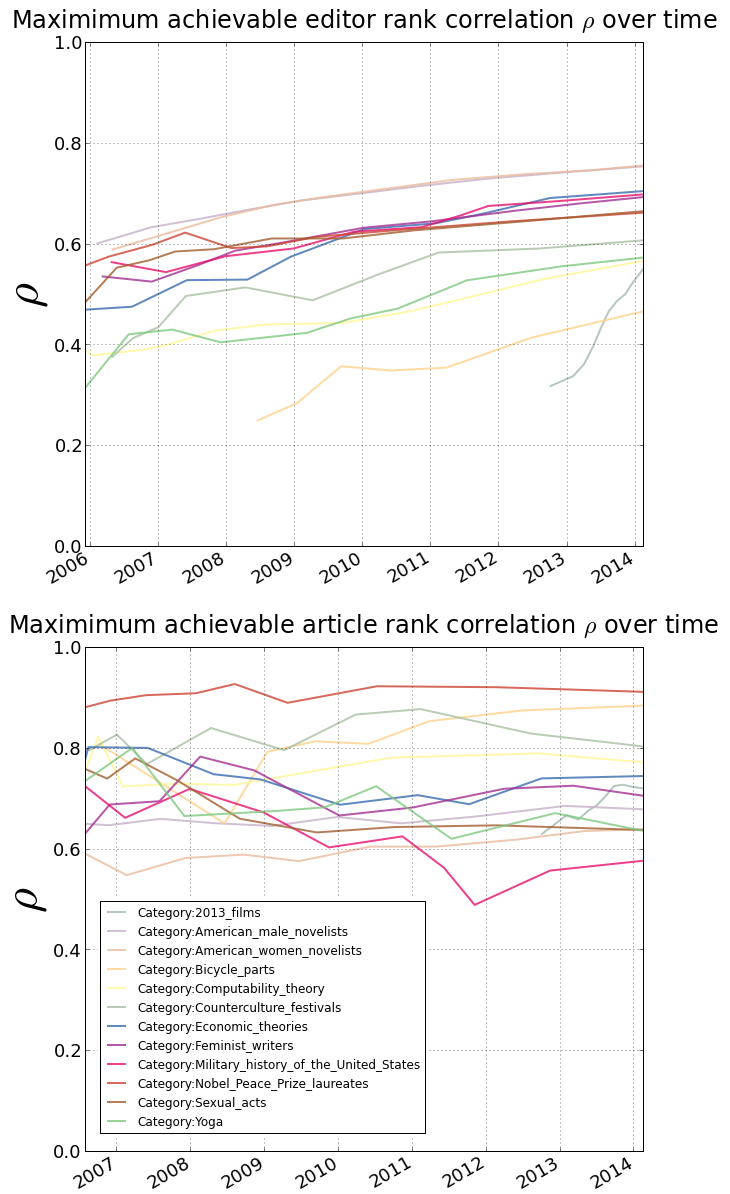
\includegraphics[width=0.9\columnwidth]{rho_combined.png}.
\caption{$\rho$ over time, by category and type}
\label{fig:rhotime}
\end{figure}


%$\alpha$ is a measure of how important it is for quality that many users edit, with lower alpha, we have a more collaborative category, where edits are more equal and egalitarean. With alpha high, the category is more rewarding users that operate more individualistically. Beta is inversely related to alpha so the same can be said but the directions of the arguments reversed. This means we can talk of the characteristic of a category, compared to one another and compared over time. 

\subsection{Negative values of $\alpha$ and $\beta$}
Another surprising result is that we find at times, negative values for $\alpha$ and $\beta$.


For editors, maximum $\rho$ always occurs strictly within a radius of 0.01 around the origin on the  $\alpha$-$\beta$ plane. The $(0,0)$ solution is significant in that it represents unbiased arithmetic averages.
\ref{fig:landscape}

For articles, the solutions have varied solutions, possibly including a negative alpha. For instance in Category Economic Theories we find a 2-dimensional solutions space of maximizing solutions with including negative values of $\alpha$ and $\beta$. \ref{fig:Figures/landscape} Why there should be this family is due optimizing solutions is due to a number of reasons. One is our use of the ranking correlation. Since we are comparing only ranks positions, there are many ways to achieve our best-prediction list and perturbing $\alpha$ and $\beta$ do not affect the rank being produced. This also means that the behaviour displayed by the  landscape indicates that one of several possibilities: That either $\alpha$ is positive but small, in which case $\beta$ is bounded tightly, which means that better editors are producing more obscure articles. Or that $\alpha$ is negative and that $\beta$ is more loosely bounded. This indicates that $\alpha$ is dominating, as is the case in equations (2). In our particular example we also find that this family is shifted towards the positive $\beta$ axis. So even as the trade off occurs, its favours $\beta$ which interpreted through equations (2) means that editors who edit relatively more obscure articles are important to success of articles in Category Economic Theories.
%move to discussionIf $\alpha$ show the importance of the fittest editors contributing, negative alpha goes to imply that in these cases its actually important that less fit editors contribute at these points. This shows anti-competetiveness. Negative beta would mean that for an editor the production of ubiquitious, common, heavily otherwise-edited articles are important. Which again is a reward for anti-competitive behaviour.

\begin{figure}[!t]
\centering
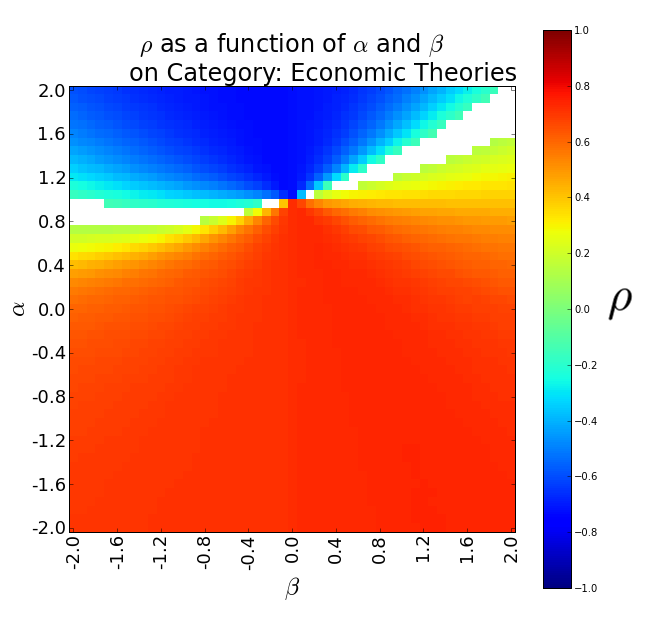
\includegraphics[width=0.9\columnwidth]{landscape.png}.
\caption{Landscape}
\label{fig:landscape}
\end{figure}




\section{Discussion}

One of the brightest results here is that in using the method described for predicting world economies by GDP, we not only can predict Wikipedia editor and article rankings, but outperform the original application. Whereas in Caldarelli the achieve a correlation of 0.4, \cite{Caldarelli} that is on the lower end of our results. A theory to explain this behaviour goes back to the original motivation in creating this method, that of trying to find "capabilities". In Economics there are circumstantial factors that influence a countries capabilities, e.g. Geography or Politics. However in Wikipedia all outputs are only due to the editors' true underlying capabilities. There are no commodities and articles have no intrinsic value until they are written. If this explained why our correlations were higher, it might also be true for other online collaboration sites, where users operate in a within a greater meritocracy.

In Wikipedia there has been discussion about the importance of super-users who represent a small fraction of editors but contribute a majority of content. \cite{website:wikinewsreporter}. It is possible now to take $\alpha$ as a measure of importance of superuser contributions. Since different categories we correlate more highly for different ranges of $\alpha$ it is possible to compare the success of super-users in different categories. Moreover we can also find which categories are most closely modelled by low or negative values of $\alpha$ which represents better articles are made by less fit editors . Ways to determine this pheonomena could be two or more power users fighting over a page can leave it worse than not being touched at all. Another is that perhaps less fit editors have a greater tendency to collaborate. Or that less fit, "newbie" editors start editing quite obvious, and there for ubiquitous articles, which have high quality already.  Whatever the reason,  it shows an anti-competitiveness. It means the contributions of less fit authors are important. This is a departure from the economics domain, where the best fits for GDP are only in the positive / positive $\alpha$-$\beta$ quadrant. 



\section{Limitations}

We do not directly measure the {\it capabilities} of editors. For instance, what does one editor do best to improve an article, among the five metrics (ratio of mark-up to readable text, number of headings, article length, citations per article length, and outgoing intrawiki links) we have used to assess the quality of an article ? 

We have not looked at the evolution of the quality of correlation as a function of iteration steps.

``less is more" : Why is it that when we incorporate more information in the matrix M, the results are not better ?

Quality of the exogenous metrics, especially for editors. It would be definitely make to look at real capabilities.

We only look at the ranking not at the real quality/expertise values ? Can we learn more the real values about the gap between articles/editors ?


%\begin{figure}
%\caption{Matrix $\mathbf{\hat{M}}$ ordered by decreasing order of edits on both contributors and articles dimensions.}
%\label{fig:matrix}
%\end{figure}
%ACKNOWLEDGMENTS are optional
%\section{Acknowledgments}

% The following two commands are all you need in the
% initial runs of your .tex file to
% produce the bibliography for the citations in your paper.
\bibliographystyle{abbrv}
\bibliography{sigproc}  

% sigproc.bib is the name of the Bibliography in this case
% You must have a proper ".bib" file
%  and remember to run:
% latex bibtex latex latex
% to resolve all references
%
% ACM needs 'a single self-contained file'!
%
%APPENDICES are optional
%\balancecolumns
%\appendix
%Appendix A
%\section{Headings in Appendices}

\end{document}

